\documentclass{standalone}
\usepackage{tikz}
\usetikzlibrary{angles,quotes}
\begin{document}
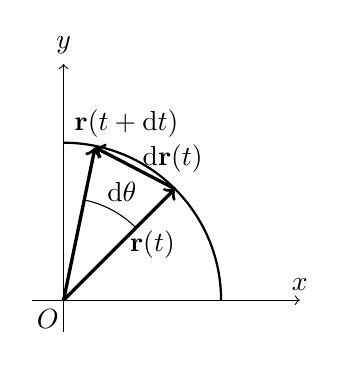
\begin{tikzpicture}[scale=2]
    \coordinate (r) at (0.707, 0.707);
    \coordinate (O) at(0,0);
    \node[below] at(-0.1, 0) {$O$};
    \draw[->] (-0.2,0)--(1.5,0)coordinate(x)node[above]{$x$};
    \draw[->] (0,-0.2)--(0,1.5)node[above]{$y$};

    \draw[->,very thick] (O)--(r) node[midway, right]{$\mathbf{r}(t)$};
    \draw[->,very thick] (O) -- (.2,0.97) coordinate(r1);
    \node[above] at (0.4,0.97) {$\mathbf{r}(t+ \mathrm{d} t)$};
    \draw[->,very thick](r)--(r1);
    \node[right] at (0.44,0.9){$\mathrm{d}\mathbf{r}(t)$};

    \draw[thick](1,0)arc(0:90:1);

    \pic["$\mathrm{d}\theta$", draw, angle eccentricity=1.2, angle radius=1.3cm]{angle=r--O--r1};
\end{tikzpicture}
\end{document}